\documentclass[12pt,spanish,letterpaper]{report}
\usepackage[spanish]{babel}
%https://ddcampayo.wordpress.com/2009/05/19/acentos-latin1-utf-8-latex/
%\usepackage[utf8x]{inputenc}
\usepackage[utf8]{inputenc}

%http://tex.stackexchange.com/questions/53470/coding-an-equation-with-description
% Descripción de las formulas
\usepackage{amsmath}
\usepackage{amssymb}
\usepackage{enumitem}

%\usepackage[total={15.5cm,22cm}, top=3cm, left=4cm]{geometry}

\usepackage[total={15.5cm,22cm}, top=2.5cm, bottom=2cm, left=3cm, right=2cm]{geometry}
\parindent = 0mm
\renewcommand{\baselinestretch}{1.1} % espaciado 1.1


\usepackage{multirow}
\usepackage{multicol}
\usepackage[table,xcdraw]{xcolor}
\usepackage{fancybox}
\usepackage{url}
\usepackage{xcolor}
%\usepackage{latexsym,amsmath,amssymb,amsfonts}
\usepackage[breaklinks,colorlinks=true,linkcolor=black, urlcolor=blue, citecolor=gray]{hyperref}


\usepackage{booktabs}
\usepackage{multirow}
%\usepackage[table,xcdraw]{xcolor}
%http://minisconlatex.blogspot.com.co/2012/01/mas-sobre-tablas-2.html
\usepackage{float} % para usar [H]

% Revisar como modificar los codigos fuente
%http://stackoverflow.com/questions/741985/latex-source-code-listing-like-in-professional-books
\usepackage{listings}
\usepackage{color}
\definecolor{mygreen}{rgb}{0,0.6,0}
\definecolor{mygray}{rgb}{0.5,0.5,0.5}
\definecolor{mymauve}{rgb}{0.58,0,0.82}


% para crear bloques de texto flotantes en la pagina
% http://tex.stackexchange.com/questions/99809/box-or-sidebar-for-additional-text
\usepackage{wrapfig}
\usepackage{tcolorbox}

%\newenvironment{WrapText}[1][r]{\wrapfigure{#1}{0.5\textwidth}\tcolorbox}{\endtcolorbox\endwrapfigure}
\newenvironment{WrapText}[1][r]{\wrapfigure{#1}{\textwidth}\tcolorbox}{\endtcolorbox\endwrapfigure}

% unas cajas mas bonitas (usa boiboites.sty)
\usepackage{boiboites}
\usepackage{amsmath}

\newboxedtheorem[boxcolor=orange, background=blue!5, titlebackground=blue!20, titleboxcolor = black]{theo}{Theorem}{anything}

\usepackage[framemethod=tikz]{mdframed}
\mdfdefinestyle{mystyle}{%
linecolor=green!70!black,outerlinewidth=1pt,%
frametitlerule=true,frametitlefont=\sffamily\bfseries\color{white},%
frametitlerulewidth=1pt,frametitlerulecolor=green!40!black,%
frametitlebackgroundcolor=green!60!black,
backgroundcolor=gray!5,
innertopmargin=\topskip,
roundcorner=5pt
}
\newmdenv[style=mystyle]{exa}
\newenvironment{example}[1]
  {\begin{exa}[frametitle=#1]}
  {\end{exa}}
  

%\selectlanguage{spanish}

%\hyphenation{ins-tru-men-tos ma-ne-ra va-rie-dad re-po-si-to-rios}

\usepackage{chngcntr}
\usepackage{graphicx}
\graphicspath{{Imagenes/}}
\counterwithout{figure}{chapter}
\counterwithout{table}{chapter}
\usepackage[tight,footnotesize]{subfigure}

%http://tex.stackexchange.com/questions/101645/how-to-turn-latex-figure-by-90-degrees-along-with-the-caption
\usepackage{adjustbox}
\usepackage{blindtext}

%resaltar texto
\usepackage{framed}
\colorlet{shadecolor}{blue!20}
% http://www.statsblogs.com/2013/05/06/colors-in-latex/

\usepackage{titlesec}
\newcommand{\hsp}{\hspace{10pt}}

\newcommand{\footcaption}[1]{\caption[#1]{#1\footnotemark.}}
\setlength\abovecaptionskip{1pt}

\titlespacing*{\chapter}{0pt}{-1cm}{0.5cm}
\titleformat{\chapter}[hang]{\Large\centering\bfseries}{\thechapter\textcolor{black}{.}\hsp}{0pt}{\Large\centering\bfseries\uppercase}
\titleformat{\section}{\large\bfseries}{\thesection}{1em}{}


\makeatletter
\renewcommand*\l@section{\@dottedtocline{2}{0em}{3.2em}}
\renewcommand*\l@subsection{\@dottedtocline{2}{0em}{3.2em}}
\renewcommand*\l@subsubsection{\@dottedtocline{2}{0em}{3.2em}}
\newenvironment{CenteredBox}{% 
\begin{Sbox}}{% Save the content in a box
\end{Sbox}\centerline{\parbox{\wd\@Sbox}{\TheSbox}}}% And output it centered
\makeatother

\ifpdf
\AtBeginDocument{
  \hypersetup{
    pdftitle = {\@title},
%pdftitle = {DRAFT}
    pdfauthor = {\@author},
    pdfsubject={\@subject},
    pdfkeywords={\@keywords}
  }
}
\fi

\AtBeginDocument{
	\renewcommand{\listfigurename}{LISTA DE FIGURAS}
	\renewcommand{\listtablename}{LISTA DE TABLAS}
	\renewcommand{\contentsname}{CONTENIDO}
	\renewcommand{\figurename}{Figura}
	\renewcommand\tablename{Tabla}
	}
	
\makeatletter
\title{Técnica de Posicionamiento GPS apoyado en interacción de dispositivos inmersos en ambientes urbanos.}\let\Titulo\@title
\author{William Javier Trigos Guevara}          \let\Autor\@author
\date{\today}           \let\Fecha\@date
\date{\year}			\let\Ano\@date


\usepackage{pdfpages}


\makeatother

\begin{document}

%\maketitle
	% -------------------------------------------------------------------------
	% Pagina de Portada
	% -------------------------------------------------------------------------
	%	\begin{titlepage}
		\begin{center}
			\textsc{\Large \textbf{Técnica de Posicionamiento GPS apoyado en interacción de dispositivos inmersos en ambientes urbanos.}}\\[8cm]

			\textsc{William Javier Trigos Guevara}\\[9cm]
			\textsc{Universidad Industrial de Santander}\\
			\textsc{Facultad de Ingenier\'ias Fisico-mec\'anicas}\\
			\textsc{Escuela de Ingenier\'ia de Sistemas e Inform\'atica}\\
			\textsc{Bucaramanga}\\	
			\the\year
		\end{center}
	\end{titlepage}
	% -------------------------------------------------------------------------
	% Pagina de Contraportada
	% -------------------------------------------------------------------------
	%	\begin{titlepage}
		\begin{center}
			%\textsc{\Large \textbf{Técnica de Posicionamiento apoyada en la interacción de dispositivos GPS inmersos en ambientes urbanos.}}\\[3.5cm]
			
			\textsc{\Large \textbf{Técnica de Posicionamiento GPS apoyado en interacción de dispositivos inmersos en ambientes urbanos.}}\\[4cm]
			
			\textsc{William Javier Trigos Guevara}\\[2.8cm]
			Trabajo de Investigación para optar por el t\'itulo de:\\[0.4cm]
			{\Large Mag\'ister en Ingenier\'ia de Sistemas e Inform\'atica}\\[3.5cm]
			Director:\\
			Ph.D Gabriel Pedraza\\[0.5cm]
			Codirector\\ 
			Raúl Ramos Pollán\\[3.0cm]
			\textsc{Universidad Industrial de Santander}\\
			\textsc{Facultad de Ingenier\'ias Fisico-mec\'anicas}\\
			\textsc{Escuela de Ingenier\'ia de Sistemas e Inform\'atica}\\
			\textsc{Bucaramanga}\\
			\the\year
		\end{center}
	\end{titlepage}

	% -------------------------------------------------------------------------
	% Tabla de Contenido
	% -------------------------------------------------------------------------
	%\setcounter{page}{3}	
	%\tableofcontents
	%\addtocontents{toc}{~\hfill\textbf{P\'ag.}\par}
	
	% -------------------------------------------------------------------------
	% Lista Figuras
	% -------------------------------------------------------------------------
	%\listoffigures
	
	% -------------------------------------------------------------------------
	% Lista de Tablas
	% -------------------------------------------------------------------------
	%\listoftables	

	% -------------------------------------------------------------------------
	% Introduccion
	% -------------------------------------------------------------------------	
	%\addcontentsline{toc}{chapter}{Introducci\'on}
	%\setcounter{page}{13}
	%\input{Capitulos/introduccion}
	
	% -------------------------------------------------------------------------
	% Objetivos
	% -------------------------------------------------------------------------	
	%\addcontentsline{toc}{chapter}{OBJETIVOS}
	%\addcontentsline{toc}{section}{Objetivo General}
	%\addcontentsline{toc}{section}{Objetivos Especificos}
	%\chapter{OBJETIVOS} 
\label{sec:objetivos}

Los objetivos planteados en este apartado tienen como propósito identificar los aspectos que permitan dar respuesta a la pregunta, ¿Es posible mejorar el nivel de precisión en localización dentro de ambientes urbanos, mediante la interacción de dispositivos de posicionamiento GPS inmersos en este ambiente?

\section{General}
Plantear una técnica de posicionamiento basada en la interacción de dispositivos GPS, para determinar si el intercambio de información entre dispositivos permite mejorar en el nivel de precisión dentro de ambientes urbanos.

% Plantear un procedimiento Diseñar una técnica de posicionamiento basado en interacción de dispositivos de posicionamiento, que contribuya a la mejora en el nivel de precisión en tareas de localización dentro de ambientes urbanos.\\


\section{Específicos}

Para alcanzar el objetivo general planteado en este trabajo de investigación, se considera importante el desarrollo de las siguientes actividades:

\begin{itemize}

\item Plantear un modelo matemático que permita construir una técnica de posicionamiento basada interacción de dispositivos GPS.

\item Validar el planteamiento matemático involucrado en la técnica de posicionamiento mediante simulación, para saber si los resultados obtenidos concuerdan con el objetivo de la investigación.

\item Seleccionar un mecanismo de interacción entre dispositivos gps, basado en la información requerida por el modelo matemático para realizar el cálculo de posicionamiento.

\item Evaluar el nivel de precisión alcanzado por los dispositivos dentro de ambientes urbanos, para identificar los casos de uso de la técnica de posicionamiento planteada.

\end{itemize}




	
	
	% -------------------------------------------------------------------------
	% Capitulos
	% -------------------------------------------------------------------------

	
	%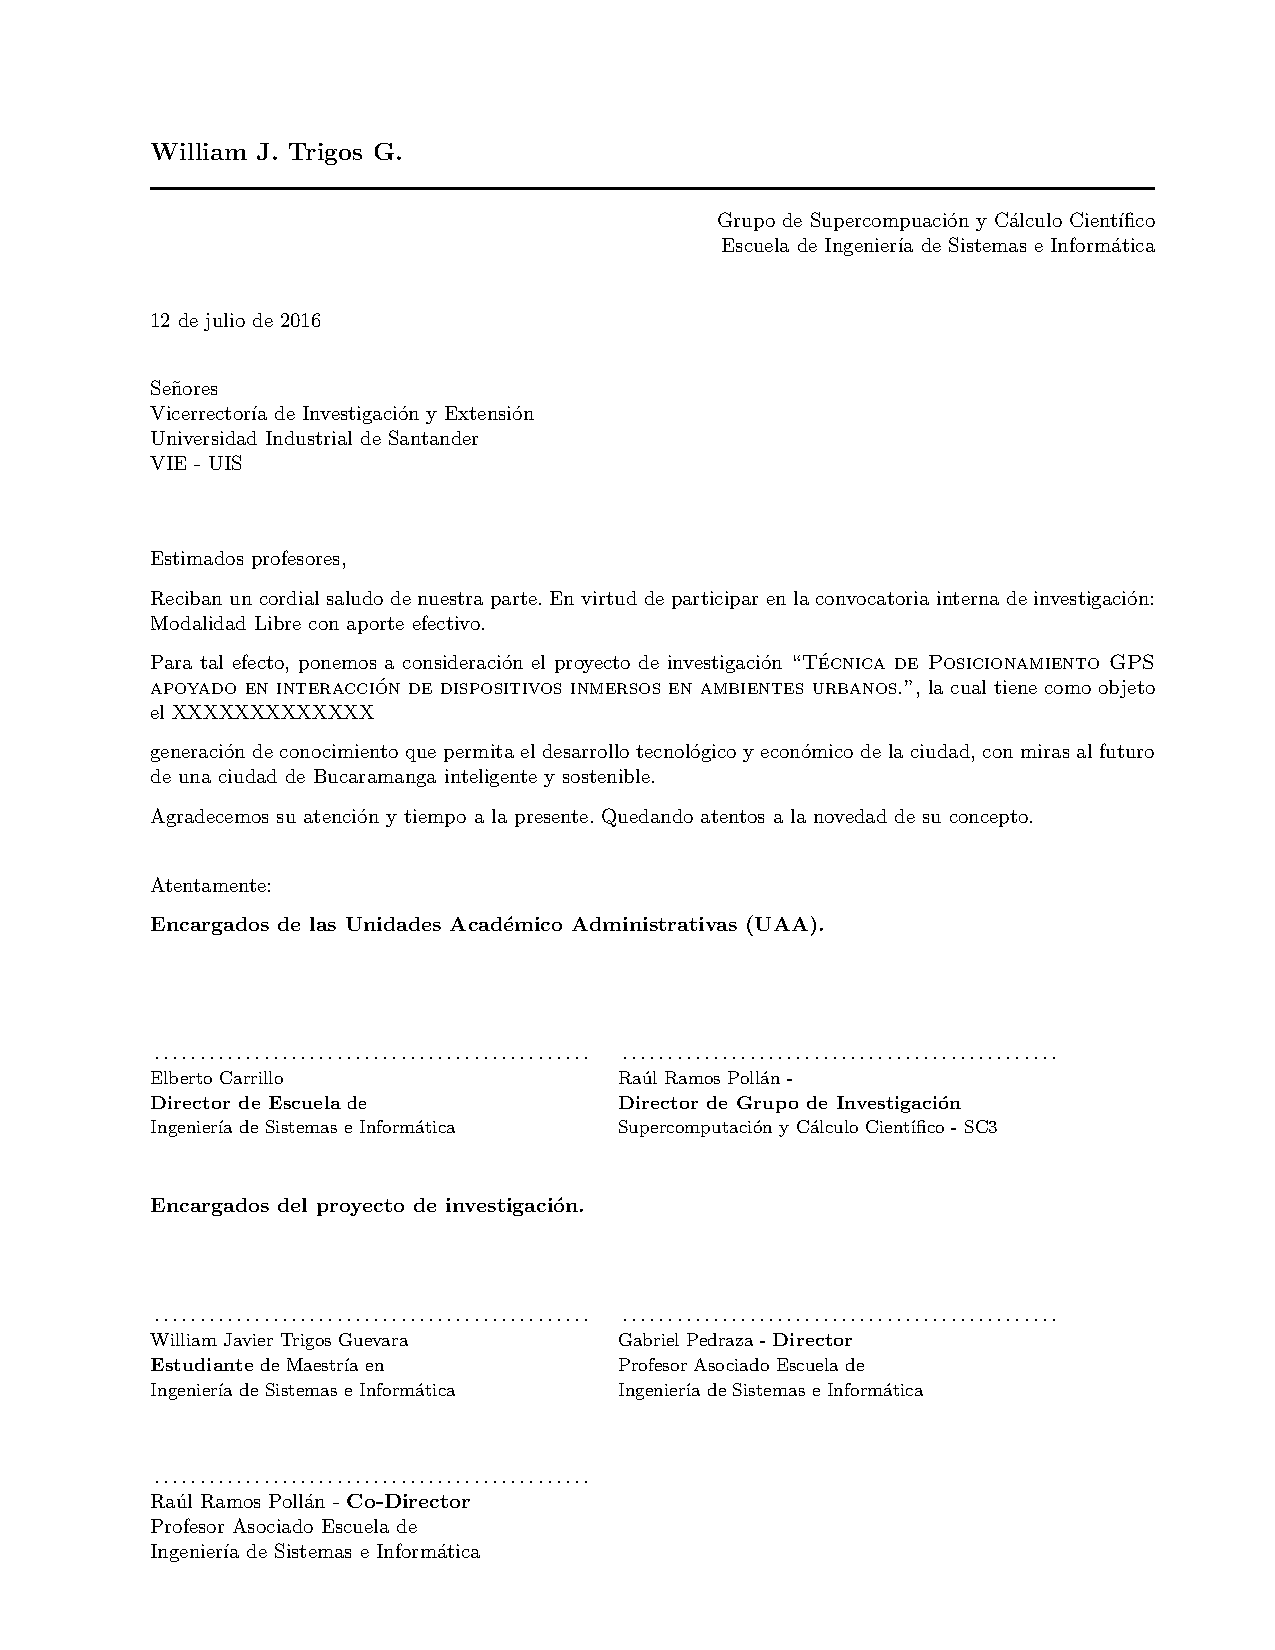
\includepdf[pages=-, scale = 0.95]{Carta_EntregaPropuesta.pdf}
	
	%	\thispagestyle{empty}
	\begin{titlepage}
		\begin{center}
			\textsc{Propuesta de Investigación:\\ Modalidad libre con aporte en efectivo.}\\[1cm]
			\textsc{\Large \textbf{Técnica de Posicionamiento apoyada en la interacción de dispositivos GPS inmersos en ambientes urbanos.}}\\[4cm]
			%\textsc{\Large \textbf{\Titulo}}\\[4cm]
			
	
			\textsc{Presentado ante:}\\
			\textsc{Vicerectoría de Investigación y Extensión}\\[3cm]
			
			\textsc{Por:}\\
			%\textsc{\Autor}\\[5cm]
			\textsc{MsC. William Javier Trigos Guevara\\
			PhD. Gabriel Rodrigo Pedraza\\
			PhD. Raúl Ramos Pollán.
			}\\[5cm]
			\textsc{Universidad Industrial de Santander}\\
			\textsc{Facultad de Ingenierías Fisico-mecánicas}\\
			\textsc{Escuela de Ingeniería de Sistemas e Informática}\\
			\textsc{Bucaramanga}\\	
			\the\year
		\end{center}
	\end{titlepage}
	%\clearpage\thispagestyle{empty}\mbox{}\clearpage
	\thispagestyle{empty}

%\chapter{Resumen}
%\section{Resumen}

\begin{center}
\Large\centering\bfseries
\textsc{RESUMEN}
\end{center}

Tras la ratificación de la eliminación de la característica de disponibilidad selectiva en futuras constelaciones GPS en 2007 %\footnote{\url{http://www.gps.gov/systems/gps/modernization/sa/}}
, se abrió paso a que los sistemas de posicionamiento satelital puedan alcansar niveles de precisión de hasta un orden de 1 metro (1m) o menos.\\

En busca de este objetivo Europa en 2011, decide hacer el lanzamiento de un nuevo sistema GNSS independiente, con capacidad de cálculo y corrección activa de orbitas y capacidad de interacción con los dos sistemas ya existentes, GLONASS(Rusia) y GPS(USA); pudiendo conformar una constelación de satélites de al menos 86 satélites funcionales en total para el 2020. Sin embargo, uno de los principales problemas de los sistemas de navegación basados en GNSS es la degradación de la precisión cuando alguno de los satélites es bloqueado, como es el caso de los edificios dentro del ambiente urbano, la vegetación espesa en zona selvática o fenómenos de interferencia entre las señales que llegan al receptor.\\

Por otra parte, se ha venido observando que a medida que la cantidad de satelites disponibles aumenta la ocurrencia de fallos en la sincronización de reloj también aumenta, afectando el nivel de precisión en posicionamiento de los receptores GNSS. El segmento de control GNSS es el encargado de monitorear y marcar los satelites que presentan errores de sincronización o estan defasados de orbitas; de esta forma estos satélites no son aptos para una buena precisión en posicionamiento.\\
% Basado en las patentes 
%	http://www.google.com/patents/US20140232595
%	https://www.google.ch/patents/US9170109

En este orden de ideas, las técnicas de posicionamiento muestran ser muy robustas en condiciones de estáticas y con buena visibilidad, la navegación dentro de las ciudades impone unas condiciones diferentes, bajo las cuales solo un monto de todos los satélites es visible. Por ello, los estudios mas recientes en sistemas de posicionamiento satelital, exploran el desarrollo de algoritmos para la detección de fallos y/o técnicas de posicionamiento para su uso dentro de ambientes urbanos, con el objetivo de alcanzar mayores niveles de precisión en posicionamiento.\\

%Una buena parte de los reportes de literatura durante la ultima década han sido enfocados a caracterizar la precisión de GPS y GNSS en ambientes a cielo abierto y urbanos, empleando dispositivos de posicionamiento estáticos. En en estos reportes se hace énfasis en el impacto que tienen la baja visibilidad de satelitales, interferencia inter-canal y el obstrucción de señales, como los factores que impiden alcanzar mayores niveles de precisión en dispositivos GPS inmersos en cañones urbanos.\\ 

%Cuando se tiene en cuenta que para 2020 habrá una gran
Teniendo en cuenta la infraestructura satelital disponible y la oferta de tecnologías y dispositivos para la recepción de señales GPS en el mercado de dispositivos electrónicos actual; surge la inquietud que que da origen a la presente investigación: \\

\textit{¿Es posible contribuir a la mejorar del nivel de precisión en posicionamiento dentro de ambientes urbanos, mediante una técnica de posicionamiento apoyada en la interacción de dispositivos GPS? y ¿Que niveles de precisión podría alcanzar esta técnica?}\\

%El contenido de este documento, es el resultado inicial del trabajo investigativo y metodológico que busca alternativas de respuesta a la pregunta de investigación planteada.\\

%El contenido de este documento, es el resultado de la inicial que tienen como objetivo el establecimiento de las bases metodológicas necesarias que permitan dar respuesta a la pregunta de investigación planteada con anterioridad.\\

%\vspace{-0.5cm}
\textbf{Key-words}:
DGPS, GNSS, GPS, Cooperative-GPS. 
\\


%\section{Presentación del documento} 

%Hasta este punto, lo que queda por resaltar de este breve recorrido histórico, es que el objetivo de llevar a cabo tareas de posicionamiento con alta precisión, es en si la premisa fundamental que argumenta el porqué de la existencia de los sistemas de posicionamiento satelital.\\

%\begin{shaded}
%El presente documento está organizado de la siguiente manera:\\
%\end{shaded}

%Primero se lleva a cabo la introducción y breve contextualización del proyecto en la sección~\ref{sec:introduccion}. La sección  \ref{sec:estadodelarte} presenta en estado del arte involucrado con la planificaci\'on de tareas sobre plataformas de cómputo de alto rendimiento y la problem\'atica del consumo energ\'etido en este tipo de arquitecturas. Luego en la secci\'on ~\ref{sec:propuesta}, se presenta de forma mas detallada la problemática, la justifcación y motivación de que sustenta la presente propuesta de investigación. En la sección~\ref{sec:objetivos} de se presenta los objetivos, alcances de la propuesta, al igual que los productos esperados de la misma.\\

%Finalmente las secciones~\ref{sec:metodologia}, ~\ref{sec:cronograma}, ~\ref{sec:Presupuesto}, presenta la metodología y cronograma de actividades el planteados para el desarrollo de la investigación junto al presupuesto necesario para el desarrollo, con lo cual se concluye el contenido de este documento de propuesta de investigación.

	
	%\clearpage\thispagestyle{empty}\mbox{}\clearpage
	\setcounter{page}{3}
	\tableofcontents
	\addtocontents{toc}{~\hfill\textbf{P\'ag.}\par}
	%\listoffigures
	%\listoftables

	
	\chapter{Marco Teórico} 
\label{sec:marcoteorico}

Este capitulo tiene como objeto introducir los conocimiento sobre sistemas de posicionamiento Global (GPS) y los aspectos técnicos relacionados con la señales y su recepción en dispositivos de posicionamiento (receptores).

\section{Sistema global de posicionamiento satelital - GNSS}

El sistema de posicionamiento global (GPS), es el primer sistema global de navegación satelital GNSS. GPS consta de una constelación de 24 satélites sobre la orbital media de la tierra que trasmite continuamente señales de radio frecuencia hacia la tierra, permitiendo así que los dispositivos de posicionamiento puedan determinar su posición sobre la superficie terrestre.\\

La idea detrás de los sistemas de posicionamiento tales como GPS, puede resumirse en que:\\

\textit{Si la distancia desde tres satélites en el espacio a un punto en común sobre la superficie de la tierra(un receptor GPS) es conocida, junto con la posición de los satélites al momento de la transmisión, la posición del receptor puede ser determinada gracias a la aplicación de conceptos trigonométricos, álgebra y un sistema de coordenadas apropiado.\cite{Thompson_1998}.}\\

Sin embargo, la problemática es ¿Como conseguir las distancias a cada satélite de forma precisa, para poder aumentar la precisión al momento de determinar la posición del receptor sobre la superficie de la tierra.?\\

Para ello es necesario profundizar mas los conceptos y conocimientos acerca del funcionamiento de GPS.

\subsection{El funcionamiento GPS}

GPS funciona gracias a la transmisión continua de señales de radiofrecuencia a través de la ionosfera y la troposfera. Las señales transmitidas están conformadas por dos señales de portadora, dos códigos y un mensaje de navegación (detalles acerca del satélite). Estas señales son adquiridas gracias una antena especialmente diseñada para captar la señales en el rango de frecuencias específicos en que transmiten los satélites GPS (1227.60 y 1575.42 MHz).\\

Posterior a la adquisición y decodificación de la señal viene una etapa de cálculos en la que un componente de software realiza cálculos para descifrar que mensaje de navegación corresponde a determinado satélite, gracias a los códigos recibidos de manera simultanea.\\


%\subsubsection
\textbf{Triangulación y trilateración.}\\

Triangulación es el método o forma más común para la  determinación de una posición sobre la superficie terrestre basada en puntos de referencias o “faros”. Para ello, los ángulos entre el receptor y los puntos de referencia deben ser conocidos para que receptor puede determinar su posición; en este escenario, la precisión con la que el receptor determina su posición, depende de la precisión con la que puede medir los ángulos con respecto a cada punto de referencia.\\
 
La Trilateración, es un método apoyado en el conocimiento de las posiciones de los puntos de referencia. En este caso, la precisión con la que el receptor puede determinar su posición depende estrictamente de la exactitud con la que puede medir la distancia hasta el punto de referencia. En este concepto se apoya el funcionamiento de GPS.

\section{Modelos observacionales y técnicas de posicionamiento}

Los observables de medición arrojado por los dispositivos de posicionamiento son el resultado de los procedimientos internos del receptor para la estimación de los tiempos de viaje de la señal, luego de las etapas de adquisición y de-modulación. Los observables entregados por los dispositivos GPS, pueden estar expresados en formato propietario(binario) o acogidos a estándares como \textbf{NMEA\footnote{NMEA: National Marine Electronics Association,  http://www.gpsinformation.org/dale/nmea.htm}} y \textbf{RINEX\footnote{RINEX: Receiver INdependent EXchange, https://igscb.jpl.nasa.gov/igscb/data/format/rinex211.txt}}.\\

%\subsection{Representación numérica de las señales}

En teoría, una vez las señales han sido decodificadas y clasificadas, con el conocimiento de las distancias de tres satélites hasta el punto donde se ubica el receptor, es posible mediante la solución a un sistema de ecuaciones que tiene como incógnitas las coordenadas X, Y, Z donde se encuentra el receptor. Sin embargo, un cuarto satélite es necesario para una cuarta variable (tiempo), la cual hace referencia al momento exacto en el que el receptor recibir las señales que le permiten posicionarse.\\

Dado que las fuentes de error a las que está expuesta la señal que viaja entre el satélite y el receptor pueden afectar la fidelidad del observable, se emplean modelos matemáticos para representar el valor medido (observable), como una expresión que contiene el valor real a medir (distancia) y la ponderación de las fuentes de error que contaminan la medición.

\subsection{Posicionamiento Autónomo %(Single Point Positioning Model)
}

Es quizás el método de posicionamiento más sencillo y autónomo que puede permitir localizar un receptor sobre la superficie de la tierra. Este método es la base inicial para llevar a cabo tareas de posicionamiento mediante GPS. El modelo SPP como comúnmente se le conoce, plantea la introducción de modelos matemáticos que representan la forma y cantidad en cómo las distintas fuentes de error afectan los observables de medición (pseudo-rango y rango de portadora).\\

El modelo de posicionamiento de punto sencillo, busca la minimización o mitigación de los errores que afectan los observables para así obtener la localización del receptor GPS o GNSS. \\%Es importante recalcar, que una de las grandes ventajas de emplear el rango de portadora como observable para tareas de posicionamiento es que el error \textbf{multipath} es mucho menor que para el observable pseudo-rango.\\

%\subsubsection
\textbf{Pseudorango.}\\

Considerando que GPS se apoya en que el cálculo de las distancias propuesto por el método de trilateración, la sincronización y precisión del tiempo en los satélites y receptor con respecto al tiempo de referencia GPS (GPSTime) es un factor importante.\\

Para ello, la sincronización de los relojes de los satélites son monitorizados por el segmento de control GPS, mientras que el reloj de los receptores es sincronizado por la recepción del los mensajes satelitales en un tiempo no mayor a 100ms, de forma que el receptor y el satélite tengan el mismo tiempo de referencia al momento del cálculo de tiempo de vuelo de la señal a través de la atmósfera y hacer posible el cálculo del pseudo-rango con un mayor nivel de precisión.\\

Una vez se cuenta con el tiempo de vuelo de la señal (TOF - time of flight), el cálculo de la %pseudo-rango 
distancia entre el satélite y el receptor puede generalizarse como:

\begin{equation}
\rho_{r}^{s} = (t_{rx} - t_{tx}) * c
\label{eq:Ec1}
\end{equation}

\noindent donde:

\begin{itemize}[label=]
	\item $c$ representa la velocidad de la luz.
	\item $t_{rx}$ tiempo al momento de la recepción, en reloj en el receptor con respecto a GPSTime.
	\item $t_{tx}$ tiempo al momento de la transmisión, en el transmisor con respecto a GPSTime.
\end{itemize}

La ecuación generalizada para el observable pseudo-rango, tomando en consideración la mayoría de las fuentes de error que la pueden afectar su correcta medición, es definida por la ecuación \ref{eq:Ec2}.

\begin{equation}
P_{r}^{s}(t) = \rho_{r}^{s}(t) +c*\tau_{r}(t) -c*\tau^{s}(t) -d_{iono}^{s} + d_{trop}^{s} + M_{r, P}^{s}(t) + \eta
\label{eq:Ec2}
\end{equation}

\noindent donde:

%http://tex.stackexchange.com/questions/53470/coding-an-equation-with-description
\begin{itemize}[label=]
	\item $P_{r}^{s}(t)$ observable de pseudo-rango, con todos los errores asociados en el proceso de adquisición de la señal.
	\item $\rho_{r}^{s}(t)$ representa el rango geométrico existente entre el receptor y el satélite en el tiempo t.
	\item $c$ velocidad de la luz.
	\item $\tau_{r}$ error asociado a la mala sincronización del reloj en el receptor con respecto al GPSTime, en el tiempo t.
	\item $\tau^{s}$ error asociado a la mala sincronización del reloj en el satélite con respecto al GPSTime, en el tiempo t.
	\item $d_{iono}^{s}$ error asociado con el retraso ionosférico.
	\item $d_{trop}^{s}$ error asociado con el retraso troposférico.
	\item $M_{r,P}^{s}(t)$ error asociado con el fenómeno de multipath en el tiempo t.
	\item $\eta$ error en la medición del pseudo-rango debido al ruido en el receptor en el tiempo t.
\end{itemize}

Es importante aclarar que para algunos modelos de observables, suele verse que los errores asociados a los orbitales de los satélites son considerados como una constante, bajo la consideración de que el cambio instantáneo en la posición de los satélites es demasiado lenta a durante el tiempo de medición, lo cual es valido para modelos simplistas y menos precisos.\\

Igualmente, el retraso ionosférico puede a ser modelados por medio de constantes o funciones con tasas de cambio lentas, para representar la variación del contenido de electrones entre una medición y otra.\\

Esta es la razón por la cual el planteamiento de las técnicas de posicionamiento diferencial, puede mitigar esta fuente de error entre mediciones consecutivas (época a época). Adicionalmente el estudio en \cite{el1994effect}, \cite{blewitt1997basics}, presenta que el retraso ionosférico para múltiples receptores ubicados relativamente cerca entre sí (rangos de 200 km), puede asumirse que el retraso ionosférico es similar para ellos.

\subsection{Posicionamiento Relativo %(Baseline Model)
}

Como su nombre lo indica, el posicionamiento relativo hace referencia a la técnica que permite localizar uno o mas dispositivos GPS con respecto a uno o más puntos referencia GPS.\\

Como se hizo referencia con anterioridad, las técnicas diferenciales pueden mitigar algunas fuentes de error que afectan la precisión en el posicionamiento; esto en virtud de manipular de los observables primarios obtenidos por el receptor, mediante la operación conocida como diferenciamiento.\\

El diferenciamiento hace referencia, a tomar la diferencia entre dos observables de medición, con el propósito de mitigar o eliminar algunas fuentes de error comunes entre estas dos mediciones.\\

%\subsubsection
\textbf{Diferenciamiento sencillo. %(Baseline Model)
}\\

El modelo de diferenciamiento sencillo, comprende la operación de diferencia entre los observables de 2 receptores (Rx1, Rx2) durante una misma epoca (mismo tiempo) con respecto a un satélite en común, como puede apreciarse en la figura \textbf{\ref{fig:SingleDifferencing}}.\\

\begin{figure}[ht]
	\centering
	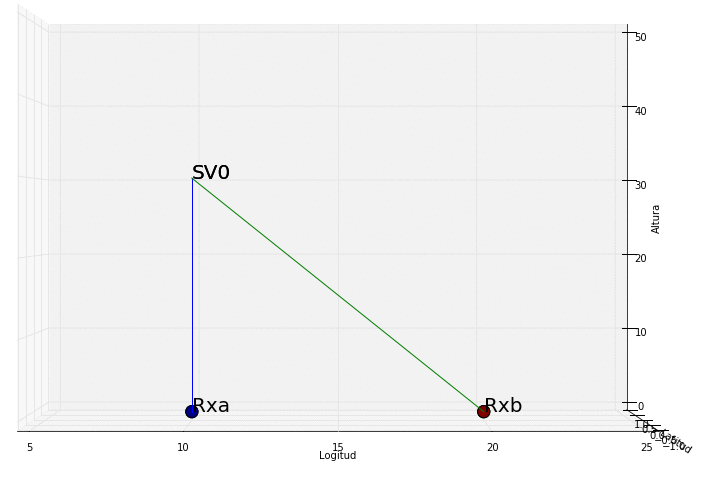
\includegraphics[scale=0.4]{Imagenes/SingleDifferencing.png}
	\caption{Diferenciamiento sencillo.}
	\label{fig:SingleDifferencing}
\end{figure}

Por términos prácticos y con el propósito de tener mayor claridad, se asume el uso del observable de medición será el pseudo-rango expresado en la ecuación \ref{eq:Ec3}. Donde el termino $\epsilon_{r}^{s}$, representa la combinación de los términos de ruido ($\eta$) y multipath ($M_{r,P}^{s}(t)$).\\ 

Los términos $d_{iono}^{s}$ y $d_{trop}^{s}$, pueden asumirse similares para ambos receptores conforme a lo expuesto en los estudios \cite{el1994effect}, \cite{blewitt1997basics}; de esta forma los observables de medición para cada receptor con respecto a un solo satélite, serían:\\

%http://tex.stackexchange.com/questions/8936/how-to-break-a-long-equation
\begin{equation}
	\begin{aligned}
		P_{A}^{s}(t) = \rho_{A}^{s}(t) +c*\tau_{A}(t) - c*\tau^{s}(t) -d_{iono}^{s} + d_{trop}^{s} + \epsilon_{A}^{s}\\
		P_{B}^{s}(t) = \rho_{B}^{s}(t) +c*\tau_{B}(t) - c*\tau^{s}(t) -d_{iono}^{s} + d_{trop}^{s} + \epsilon_{B}^{s}
	\label{eq:Ec3}
	\end{aligned}
\end{equation}\\

La operación de diferenciamiento entre los observables presentados en la ecuación \ref{eq:Ec3}, se define como $\bigtriangleup P_{AB}^{s}$:\\

\begin{equation}
	\begin{aligned}
		\bigtriangleup P_{AB}^{s} 
		& = P_{B}^{s} - P_{A}^{s}\\
		& =(\rho_{B}^{s}-\rho_{A}^{s}) + c*(\tau_{B} - \tau_{A}) + (\epsilon_{B}^{s} - \epsilon_{A}^{s})\\
		& = \bigtriangleup \rho_{AB}^{s} + c*\bigtriangleup (\tau_{AB}) + \bigtriangleup(\epsilon_{AB}^{s})
	\label{eq:Ec4}
	\end{aligned}
\end{equation}\\


%\subsubsection{
\textbf{Doble diferenciamiento.}\\

El modelo de doble diferenciamiento, también conocida como "diferenciamiento entre satélites"\cite{van2008gps} - es el diferenciamiento entre dos diferenciales sencillos según lo define, con lo que básicamente se encuentra la diferencia entre las observaciones de 2 receptores con respecto a un par satélites.\\

\begin{figure}[ht]
	\centering
	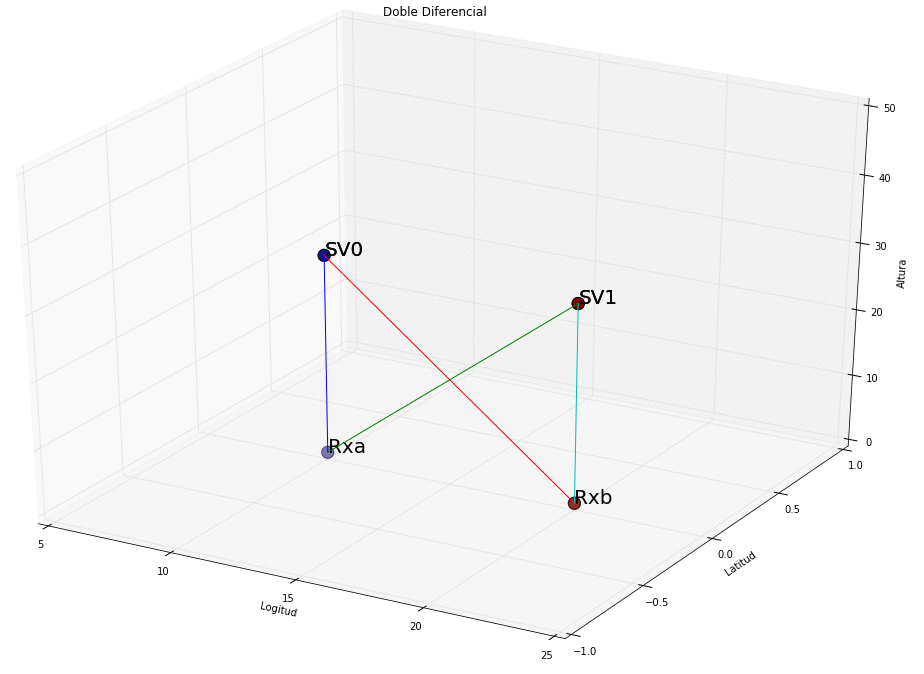
\includegraphics[scale=0.4]{Imagenes/DoubleDifferencing.png}
	\caption{Doble diferenciamiento.}
	\label{fig:DoubleDifferencing}
\end{figure}

Retomando la ecuación ~\ref{eq:Ec4}, que es el resultado entre el diferenciamiento de los observables de un receptor A y B con respecto a un satélite y considerando el escenario de la figura \textbf{\ref{fig:DoubleDifferencing}}, se tiene que:

\begin{equation}
	\begin{aligned}
		\bigtriangledown\bigtriangleup P_{AB}^{12} 
		& = \bigtriangleup P_{AB}^{2} - \bigtriangleup P_{A}^{1}\\
		& = \bigtriangleup \rho_{AB}^{12} + \bigtriangleup\epsilon_{AB}^{12}
	\label{eq:Ec5}
	\end{aligned}
\end{equation}

Donde el símbolo $\bigtriangledown$ representa la segunda operación de diferenciamiento con respecto a un segundo satélite en común entre los receptores A y B.\\

Según se expresa en la ecuación \ref{eq:Ec5}, al desarrollar la operación de doble diferenciamiento, los términos asociados con la mala sincronización en los relojes de los satélites y los receptores, son eliminados. Quedando el término $\epsilon_{r}^{s}$, quien representa la combinación de los términos de ruido ($\eta$) y multipath ($M_{r,P}^{s}(t)$).

%% Pag 36 Documento Relative Positioning

% Debido a que pueden existir tantas operaciones de doble diferenciamiento como tantos pares de receptores tengan pares de satélites en común, es probable que los resultados de la aplicación de doble diferenciamiento puedan ser una combinación lineal de sus semejantes; generando información inútil para llevar a cabo la tarea de posicionamiento.\\

% Para evitar este inconveniente la creación de un receptor y un satélite de referencia, sobre los cuales se tienen operaciones de doble diferenciamiento que arrojan resultados de observables que son linealmente independientes.\\

%Sin embargo para garantizar la selección de un receptor de referencia apropiado entre todos los disponibles, lo ideal es seleccionar aquel que tiene mayor visibilidad a satélites y a los demás receptores que lo rodean, de forma que sus semejantes se puedan beneficiar de él para realizar correcciones en sus observables; considerando que este receptor de referencia por tener mejor visibilidad de satélites, el error asociado al fenómeno de multipath se ve minimizado.\\ 

% En cuanto a la elección del satélite de referencia, el seleccionar el satélite con mayor elevación entre la lista de satélites comunes entre los receptores, de forma que este puede ser visto desde a todos ellos y además les garantiza que el efecto multipath y retraso atmosférico (ionosférico y troposférico) son reducidos.\\
	\chapter{Estado del Arte}
\label{sec:estadodelarte}

En calidad de abordar la búsqueda de precisión decimétrica en sistemas de posicionamiento, se ha realizado un breve recorrido por la literatura para clasificar aquellos trabajos que se consideran relevantes para el desarrollo de la presente investigación.\\ 

Producto de la revisión de los trabajos desarrollados durante las últimas dos décadas y relacionados con temas de interés para le presente investigación, se considera la clasificación de los mismos en 3 grandes grupos. \\

En el primer grupo a considerar, se encuentran los trabajos relacionados con el modelado matemático y representación de fenómenos relacionados con el comportamiento de la ionosfera, troposfera durante el viaje de la señal desde el satélite al receptor, así como el planteamiento de modelos corrección y predicción de orbita de satélites y/o errores por efectos de reflexión y difracción, que tienen incidencia el nivel de precisión en tareas de localización y posicionamiento. \\

Un segundo grupo, es el orientado a la mejora y desarrollo de aplicaciones GNSS apoyado en la integración de tecnologías emergentes y la tecnología GNSS, para aplicaciones civiles, comerciales y científicas, como son los casos de integración de unidades de medición inercial (IMU) con GPS, Indoor-GPS, Outdoor-GPS, etc, en sistemas de transporte inteligente (ITS), medición del desplazamiento de capas tectónicas, medición de nivel de cauce en ríos y lagos, entre otros.\\

Dentro de este grupo, los estudios relacionados van desde el estudio patrones de movimiento de la población dentro de mercados ambulantes \cite{Tsang_2011}, atractivos turísticos y zonas de reserva natural \cite{Meijles_2014}, \cite{Orellana_2012}; hasta el desarrollo de un sistemas de posicionamiento cooperativos para sistemas de trasporte inteligente (ITS) dentro de ambientes urbanos \cite{Tang_2014}.\\

Finalmente una publicación que presenta una interesante visión del futuro de la tierra basada el uso de Internet de la cosas (IOT) \cite{Li_2014}. Se propone una completa infraestructura apoyada en dispositivos móviles, que trabajan como sensores y entregan información a un servicio web encargado de generar modelos de información locales y globales. Con la información presentada mediante modelos de información 3D, tendrían información útil para la prevención de desastres naturales, pronostico del clima y estudios de fenómenos geológicos.\\  

Todas las áreas presentadas en esta clasificación tienen una característica u objetivo en común y es que, con el aporte de cada uno de ellos lo que se busca es tener un posicionamiento de precisión. 

\begin{figure}[h]
	\centering
    \subfigure[Palabras Claves.]{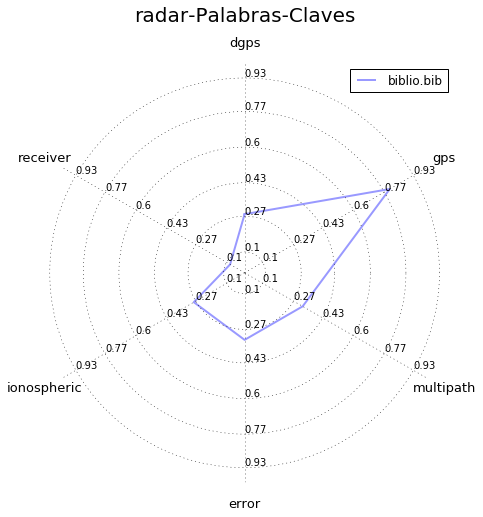
\includegraphics[scale=0.4]{Imagenes/ReporteBiblio/radar-Palabras-Claves.png}}
    \subfigure[Tipos de Documento.]{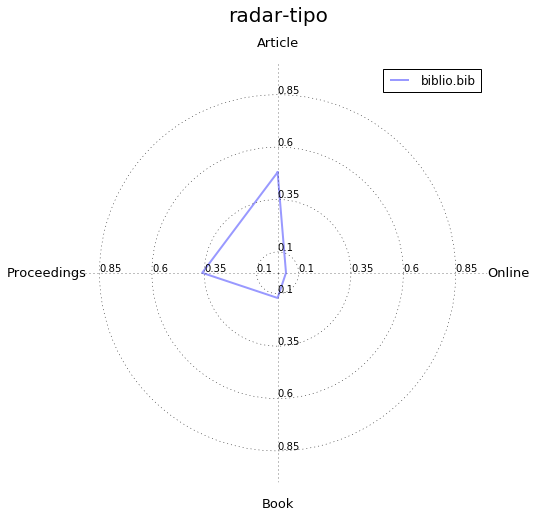
\includegraphics[scale=0.4]{Imagenes/ReporteBiblio/radar-tipo.png}}
	\caption{Extracción de información desde Estado del arte.}
	\label{fig:EstadoArte1}
\end{figure}

Los valores presentados en la Figura \ref{fig:EstadoArte1}, corresponden a valores porcentuales producto de la revisión de un total de 30 documentos, para llevar a cabo el planteamiento de la presente propuesta.\\

En listado de palabras presentado en la Figura \ref{fig:Relativewords}, es producto de la asociación de la palabras claves encontradas en cada articulo revisado, que dan idea de los temas que pueden estar relacionados con el objeto de esta investigación y que permiten tener una idea del contexto y trabajos relacionados con la misma. 

\begin{figure}[h]
	\centering
    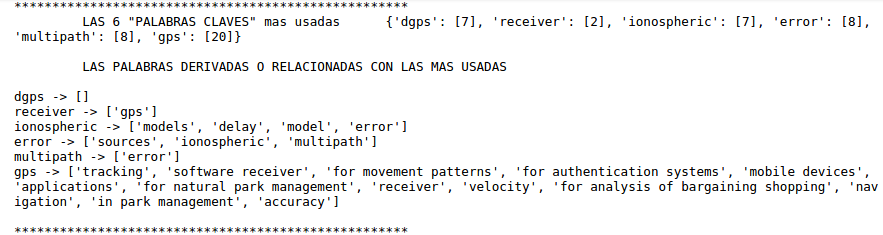
\includegraphics[scale=0.5]{Imagenes/ReporteBiblio/Relative_words.png}
	\caption{Palabras derivadas o relacionadas con las palabras claves de los artículos revizados.}
	\label{fig:Relativewords}
\end{figure}





	\chapter{OBJETIVOS} 
\label{sec:objetivos}

Los objetivos planteados en este apartado tienen como propósito identificar los aspectos que permitan dar respuesta a la pregunta, ¿Es posible mejorar el nivel de precisión en localización dentro de ambientes urbanos, mediante la interacción de dispositivos de posicionamiento GPS inmersos en este ambiente?

\section{General}
Plantear una técnica de posicionamiento basada en la interacción de dispositivos GPS, para determinar si el intercambio de información entre dispositivos permite mejorar en el nivel de precisión dentro de ambientes urbanos.

% Plantear un procedimiento Diseñar una técnica de posicionamiento basado en interacción de dispositivos de posicionamiento, que contribuya a la mejora en el nivel de precisión en tareas de localización dentro de ambientes urbanos.\\


\section{Específicos}

Para alcanzar el objetivo general planteado en este trabajo de investigación, se considera importante el desarrollo de las siguientes actividades:

\begin{itemize}

\item Plantear un modelo matemático que permita construir una técnica de posicionamiento basada interacción de dispositivos GPS.

\item Validar el planteamiento matemático involucrado en la técnica de posicionamiento mediante simulación, para saber si los resultados obtenidos concuerdan con el objetivo de la investigación.

\item Seleccionar un mecanismo de interacción entre dispositivos gps, basado en la información requerida por el modelo matemático para realizar el cálculo de posicionamiento.

\item Evaluar el nivel de precisión alcanzado por los dispositivos dentro de ambientes urbanos, para identificar los casos de uso de la técnica de posicionamiento planteada.

\end{itemize}




	
	\chapter{Metodología}

Con el fin de alcanzar los objetivos planteados en este proyecto de investigación, se reconoce la necesidad de fijar una secuencia y prioridad de actividades. Por ello de se proponen las fases de desarrollo para el proyecto, cada una de las cuales tiene finalidad y funcionalidad dentro del desarrollo del proyecto de investigación. Con fines de realizar control y seguimiento a cada una de las fases, se plantea un cronograma de actividades con intervalos de tiempo conformes a las cargas de trabajo de las actividades a realizar.\\

A continuación se presenta una perspectiva global del proyecto y la descripción de las actividades a desarrollar, para lograr los objetivos propuestos para el proyecto.

%%
	\begin{figure}[ht]
		    \centering
		    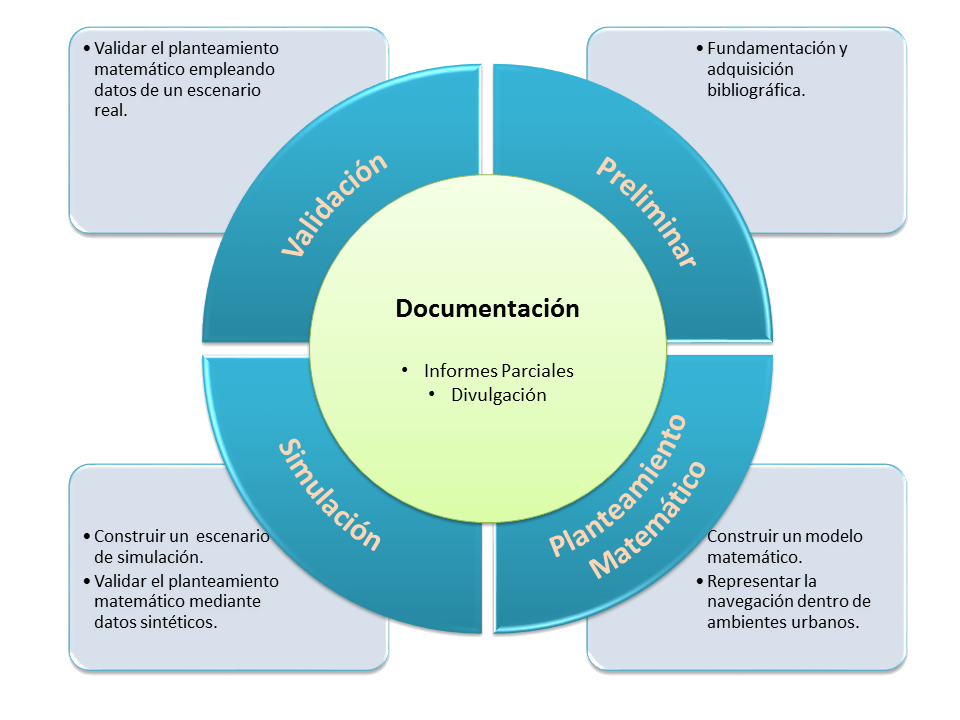
\includegraphics[scale=0.42]{Metodologia.png}
		    \caption{Metodología para el desarrollo del proyecto.}
		    \label{fig:Metodologia}
	\end{figure}


% La metodología a seguir consta de las siguientes fases:

\section{Fundamentación y adquisición bibliográfica}

Durante el transcurso de las cinco (5) semanas iniciales del proyecto (de las 16 destinadas para el desarrollo total); serán destinadas a la contextualización y consulta bibliográfica acerca de sistemas embebidos, procesadores embebidos, modelos de programación y plataformas de cómputo de alto rendimiento; con el fin de tener bases y fundamentos teóricos para enfocar el futuro inmediato del proyecto.\\

Como son el planteamiento del modelo matemático para la técnica de posicionamiento y la selección de un medio de comunicación entre dispositivos para el intercambio de información en materia de observables de posicionamiento.

\section{Construcción del prototipo software}

Esta etapa comprende el desarrollo de una versión simulada de la técnica de posicionamiento, que acoge los planteamientos matemáticos y modelos numéricos considerados necesarios para representar %de la mejor forma 
las condiciones en que se ve involucrado un dispositivo de posicionamiento durante la tarea de posicionamiento dentro de un ambiente urbano.\\

Con el prototipo de software construido se procede a verificar los  resultados numéricos del mismo, con los cuales se tiene un %considerarse como (permiten tener ) 
primer acercamiento al comportamiento y características de la técnica desarrollada; sobre los cuales se puede ejercer criterio y determinar si el planteamiento matemático producto de la fase anterior, es un recurso valido para el alcance del objetivo planteado en la presente propuesta de investigación.

\section{Construcción del prototipo hardware}

Con la ayuda del prototipo de software y los resultados de simulación del planteamiento matemático, se identificará el tipo de información y  medio de comunicación requerido para el intercambio de información entre dispositivos, que permita a la técnica de posicionamiento planteada llevar a cabo el cálculo y solución del posicionamiento del dispositivo que lo emplee.\\

Igualmente se lleva a cabo la integración del software y los  componentes de hardware disponibles, para la creación de receptores GPS con los cuales obtener datos bajo condiciones reales de la técnica de posicionamiento propuesta.

\section{Fase de análisis de caso de estudio}

Con esta actividad se busca clasificar lo datos obtenidos por los receptores GPS al momento de emplear la técnica de posicionamiento propuesta, con el fin de evaluar el nivel de precisión obtenido en escenarios al aire libre y dentro de cañones urbanos.\\

Con base en estos resultados, se busca construir argumentos y conclusiones suficientes para determinar si la técnica de posicionamiento propuesta es una alternativa de solución a la problemática planteada y permite dar respuesta a la pregunta de investigación bajo la cual se origina este trabajo de investigación.

%se pretende hacer un análisis global de la técnica con el fin de identificar deficiencias y mejoras de la misma, que puedan dar paso a trabajos futuros, así también conclusiones


\section{Fase de divulgación}

Durante el desarrollo de cada una de las fases que componen la metodología propuesta, se generan controles de avance del proyecto junto con procesos de redacción y revisiones parciales del documento final; donde se materializa experiencia adquirida y los resultados alcanzados durante cada fase de la investigación.\\

Esta fase de la investigación esta enfocada a la divulgación de los resultados y experiencias adquiridas por medio de una publicación científica; en conformidad a lo definido en el reglamento de general posgrados \footnote{Articulo 114 (numeral c): \textit{En el caso de maestrías de investigación, haber publicado o tener la aprobación para la publicación de un (1) artículo de su autoría, en una revista científica indexada u homologada por Colciencias o con índice de impacto o haber participado con ponencia en, al menos, un (1) evento académico internacional en el campo disciplinar de la maestría.},  Acuerdo 075 de 2013 - Consejo Superior - Univ. Industrial de Santander.},para la obtención del titulo profesional como Magíster en Ingeniería de Sistemas. 
	\chapter{Cronograma de actividades}
\label{sec:cronograma}


El cronograma de actividades correspondiente a esta propuesta de investigación se describe a continuación:

\begin{figure}[ht]
	\begin{adjustbox}{addcode={
		\begin{minipage}{\width}}{%
			\caption{Cronograma de actividades propuesto para el desarrollo del presente proyecto de investigación [Fuente: Autor]}
		\end{minipage}},rotate=90,center}
      	%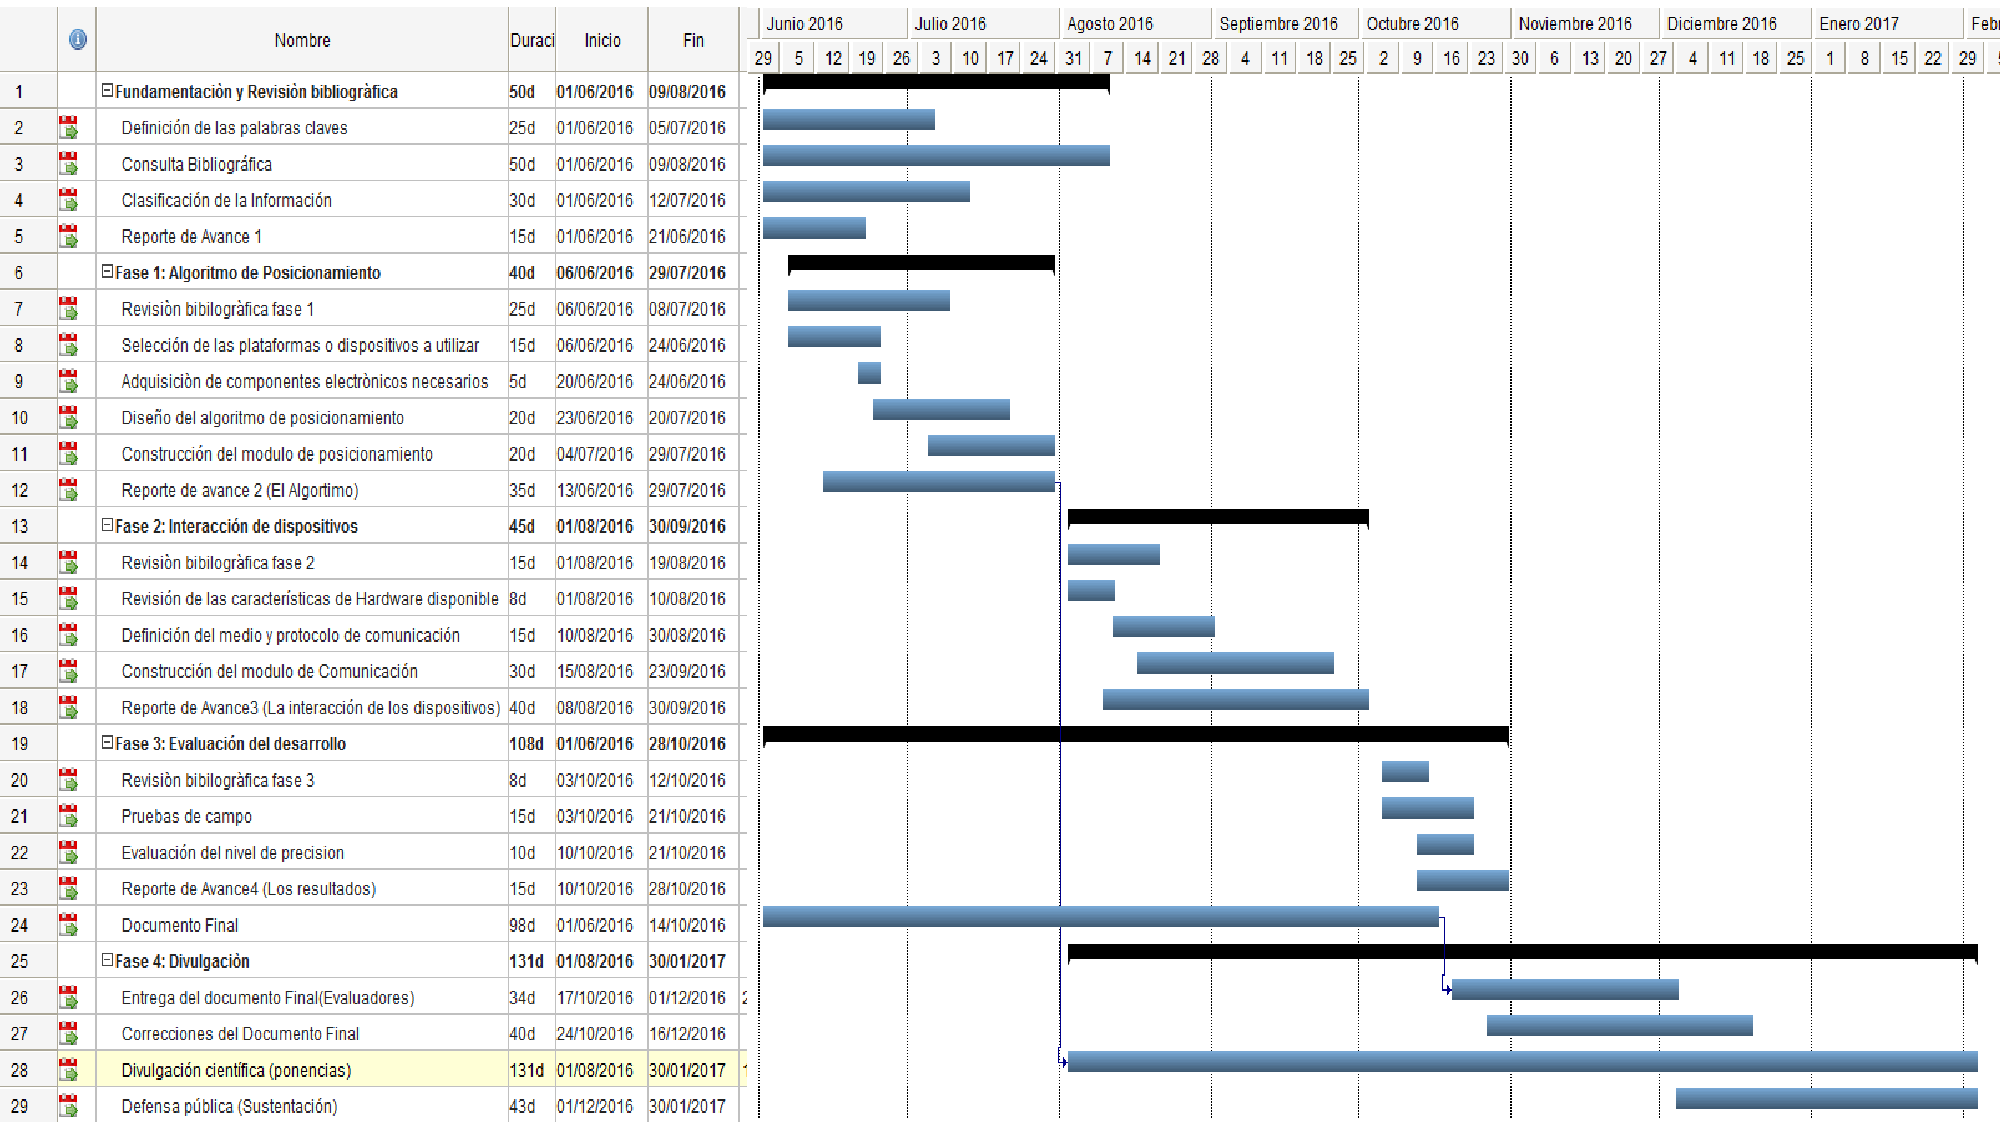
\includegraphics[scale=.40] {Imagenes/Gantt_GNSS}%
      	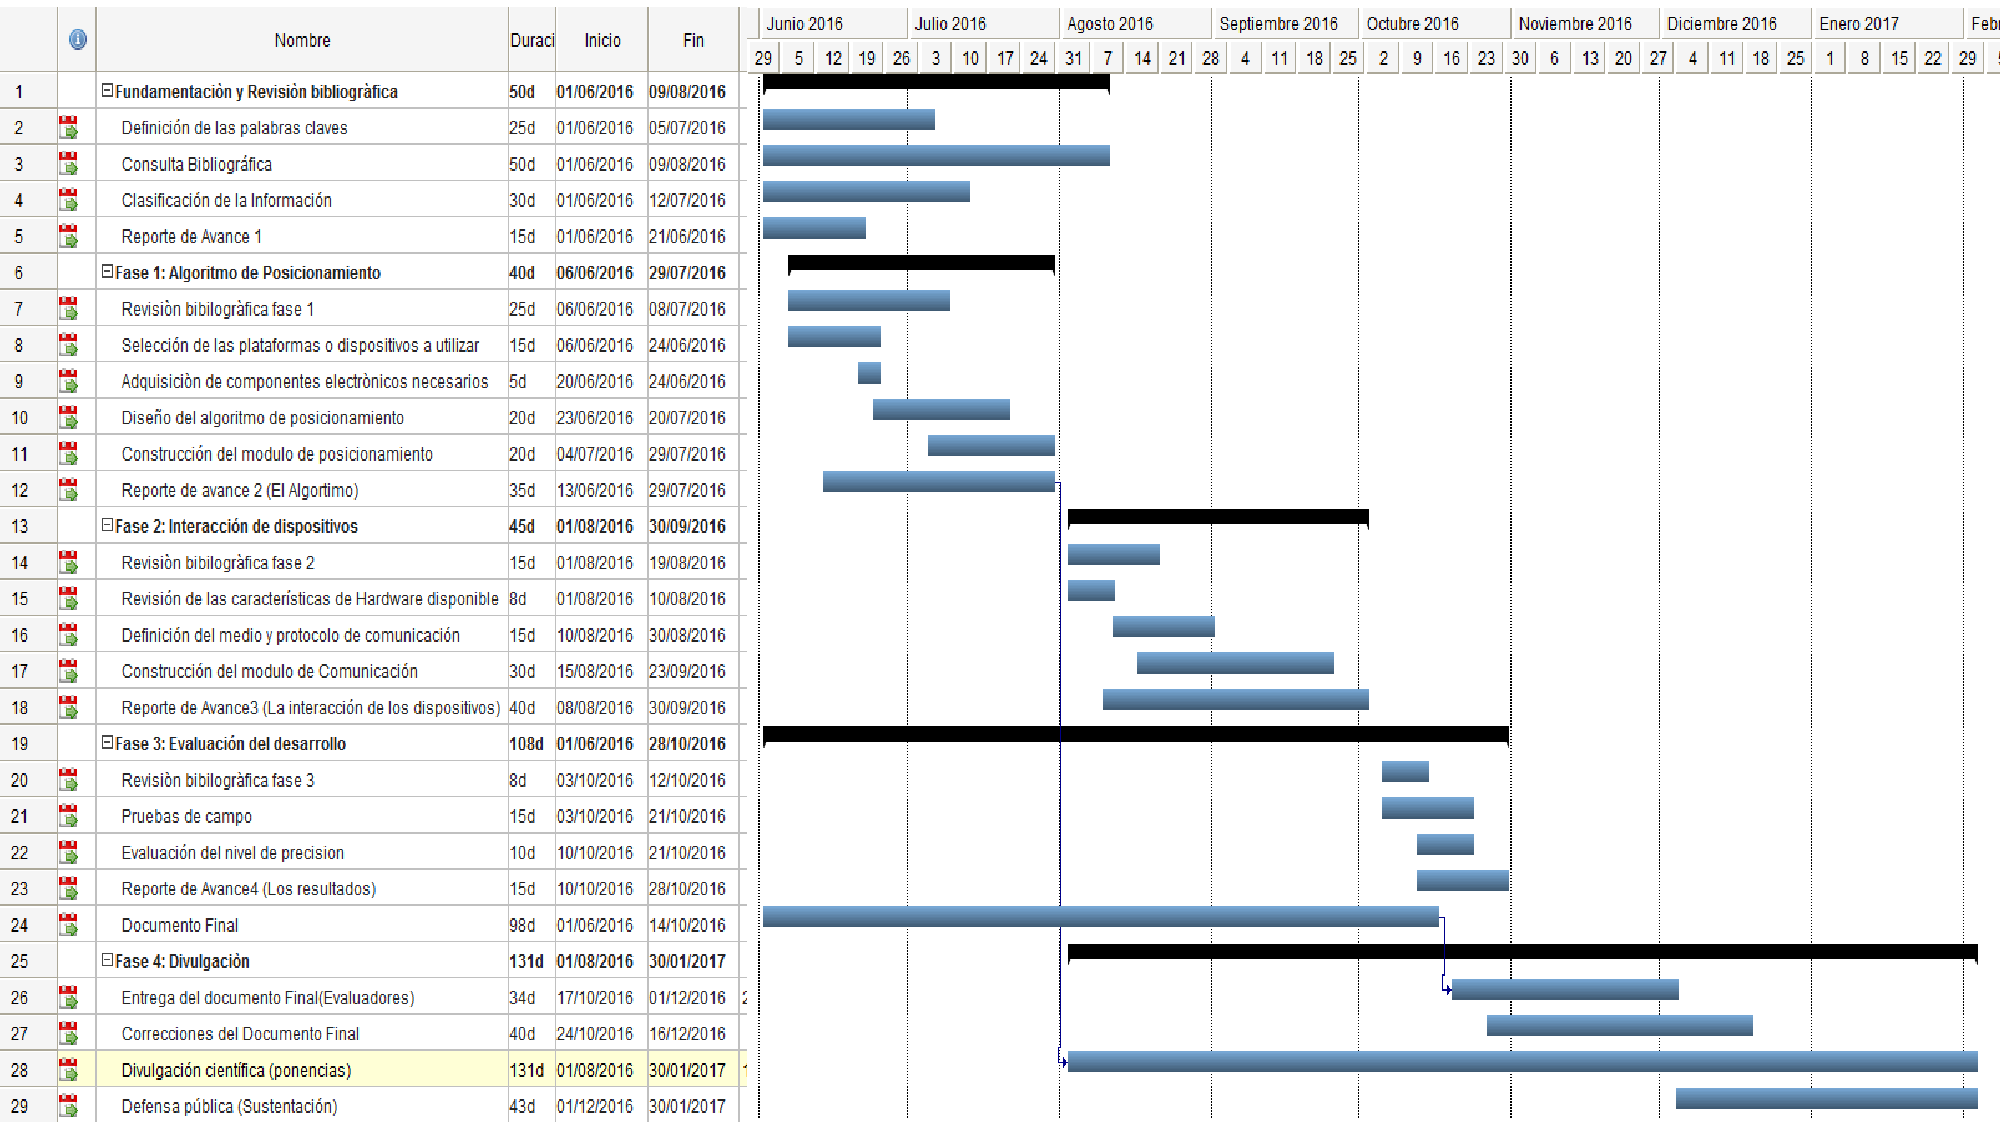
\includegraphics[scale=.5] {Imagenes/Gantt_GNSS.pdf}%
  	\end{adjustbox}
\end{figure}
	\chapter{Presupuesto}
\label{sec:Presupuesto}

Con el fin de cuantificar los recursos necesarios para el desarrollo de este trabajo, se presentan de forma detallada los costos relacionados con cada uno de los recursos utilizados para la ejecución del proyecto, y los costos adicionales generados por imprevistos.\\

\section{Equipos y dispositivos}

\begin{table}[htbp]

	\begin{center}

  	\resizebox{\linewidth}{!}{

    %http://tex.stackexchange.com/questions/31672/column-and-row-padding-in-tables
    \setlength{\tabcolsep}{0.2cm}
    %\setlength{\tabcolsep}{0.5em} % for the horizontal padding
        {\renewcommand{\arraystretch}{1.3}% for the vertical padding
        
		\begin{tabular}{p{2cm} p{5cm} p{2cm} p{2cm} p{2cm} p{3cm}}
			\hline
				\multicolumn{6}{c}{\multirow{3}{*}{\textbf{Dispositivos y Equipos  Electrónicos}}}	\\
				\multicolumn{6}{c}{}\\ 
				\multicolumn{6}{c}{}\\ 
			\hline
				\textbf{Naturaleza}	& \textbf{Componente} & \textbf{Unidad} & \textbf{Cantidad} & \textbf{Valor Unitario} & \textbf{Subtotal}\\
			\hline				
				\multicolumn{1}{c}{\multirow{2}{*}{\textbf{Equipos de Computo**}}} & 
				PCs Personales & Hora/Uso & 640 & 1,803 & \$ 1,153,846 \\
				\multicolumn{5}{c}{\textbf{Subtotal 1}} & \$ 1,153,846 \\ 
			\hline	
				\multirow{7}{*}{\textbf{Equipos y suministros }} &  %electrónicos adicionales
				Módulo GPS/GNSS					& Hora/Uso		& 2 & \$ 95,702	& \$ 191,404 \\
				{} & Router inalámbrico Gigabit & Hora/Uso		& 1 & \$ 89,322 & \$ 89,322 \\
				{} & Tarjetas Embebidas 		& Dispositivo	& 2 & \$ 596,160 & \$ 1,192,320 \\
				{} & Cargadores 				& Dispositivo	& 2 & \$ 99,360 & \$ 198,720 \\
				{} & Memorias SD				& Dispositivo	& 4	& \$ 31,050 & \$ 124,200 \\
			\hline
			\multicolumn{5}{c}{\textbf{Costo Parcial}}											& \$ 1.659.346\\
			\hline	
			\multicolumn{5}{c}{\multirow{1}{*}{\textbf{Costos de Impuestos y Envío  (24\%)}}} 	& \$ 398.243\\
			\multicolumn{5}{c}{\multirow{2}{*}{\textbf{Subtotal 2}}}            & \multirow{2}{*}{\$ 2.057.589} \\
			\multicolumn{6}{c}{} \\ 
			\hline
			\multicolumn{4}{c}{**Los costos indicados en esta tabla registran para el año 2016; pueden estar sujetos a modificación} & \multirow{2}{*}{\textbf{\$Total}} &                       \multirow{2}{*}{\textbf{\$ 3.211.435}} \\
			\multicolumn{6}{c}{} \\ 
			\hline
		    \end{tabular}%
        }
	}
	\end{center}
	
	\caption{Dispositivos y Equipos  Electrónicos}
	\label{Tabla1}
\end{table}

\section{Insumos de papelería, Consultas Bibliográficas y Costos de divulgación.}

En la siguiente tabla se describen los costos relacionados con insumos de papelería y costos de viáticos considerados para la presente investigación.\\

\begin{table}[tb]

	\begin{center}

  	\resizebox{\linewidth}{!}{

    %http://tex.stackexchange.com/questions/31672/column-and-row-padding-in-tables
    \setlength{\tabcolsep}{0.2cm}
    %\setlength{\tabcolsep}{0.5em} % for the horizontal padding
        {\renewcommand{\arraystretch}{1.3}% for the vertical padding
        
		\begin{tabular}{p{2cm} p{5cm} p{2cm} p{2cm} p{2cm} p{3cm}}
			\hline
				\multicolumn{6}{c}{\multirow{3}{*}{\textbf{Insumos, Consultas Bibliográficas y Costos de divulgación.}}}	\\
				\multicolumn{6}{c}{}\\ 
				\multicolumn{6}{c}{}\\ 
			\hline
				\textbf{Naturaleza}	& \textbf{Componente} & \textbf{Unidad} & \textbf{Cantidad} & \textbf{Valor Unitario} & \textbf{Subtotal}\\
			\hline				
				\multicolumn{1}{c}{\multirow{2}{*}{\textbf{Consultas*}}} & 
				Consultas Bibliográficas 	& Hora 			& 1680 	& 1000 		& \$ 1.680.000 \\
				\multicolumn{1}{c}{\multirow{2}{*}{}} & 
				Accesos a Base de Datos 	& Consulta 		& 150 	& 7.800 	& \$ 1.170.000 \\
				\multicolumn{5}{c}{\textbf{Subtotal 1}}  						& \$ 2.850.000 \\ 
			\hline	
				\multicolumn{1}{c}{\multirow{2}{*}{\textbf{Papelería*}}} &  %electrónicos adicionales
				Impresiones 				& Unidad		& 800	& \$ 100	& \$ 80.000 \\
				{} & Fotocopias 			& Unidad		& 400  	& \$ 50 	& \$ 40.000 \\
				{} & Empastes y Digitación 	& Unidad		& 2 	& \$ 60.000 & \$ 120.000 \\
				\multicolumn{5}{c}{\textbf{Subtotal 2}}  						& \$ 220.000 \\ 
			\hline	
				\multicolumn{1}{c}{\multirow{2}{*}{\textbf{Software*}}} &  %electrónicos adicionales
				Ofimatica 					& Hora/Uso		& 4.300 & \$ 0 		& \$ 0 \\
				\multicolumn{5}{c}{\textbf{Subtotal 3}}  						& \$ 0 \\ 
			\hline	
				\multicolumn{1}{c}{\multirow{2}{*}{\textbf{Divulgación*}}} &  %electrónicos adicionales
				Pasajes 					& Ponencia	& 1 & \$ 1.552.500 		& \$ 1.552.500 \\
				{} & Viáticos 				& Ponencia	& 1 & \$ 1.397.250 		& \$ 1.397.250 \\
				\multicolumn{5}{c}{\textbf{Subtotal 4}}  						& \$ 2.949.750 \\ 
				
			\hline
			\multicolumn{5}{c}{\textbf{Costo Parcial}}							& \$ 6.019.750\\
			\hline	
			\multicolumn{5}{c}{\multirow{1}{*}{\textbf{Costos de Impuestos y Envío  (24\%)}}} 	& \$ 1.444.740\\
			%\multicolumn{5}{c}{\multirow{2}{*}{\textbf{Subtotal 2}}}       	    & \multirow{2}{*}{\$ 7.464.490} \\
			%\multicolumn{6}{c}{} \\ 
			\hline
			\multicolumn{4}{c}{**Los costos indicados en esta tabla registran para el año 2016; pueden estar sujetos a modificación} & \multirow{2}{*}{\textbf{\$Total}} &             \multirow{2}{*}{\textbf{\$ 7.684.490}} \\
			\multicolumn{6}{c}{} \\ 
			\hline
		    \end{tabular}%
        }
	}
	\end{center}
	
	\caption{Dispositivos y Equipos  Electrónicos}
	\label{Tabla1}
\end{table}

\section{Recurso Humano}

\begin{table}[H]
	\begin{center}

  	\resizebox{\linewidth}{!}{

    %http://tex.stackexchange.com/questions/31672/column-and-row-padding-in-tables
    \setlength{\tabcolsep}{0.3cm}
    %\setlength{\tabcolsep}{0.5em} % for the horizontal padding
        {\renewcommand{\arraystretch}{1.2}% for the vertical padding
        
			\begin{tabular}{p{4.5cm}p{2.5cm}p{2.5cm}p{2.2cm}p{1.7cm}p{3cm}p{3cm}}
			 \hline
			 \multicolumn{7}{c}{\multirow{3}{*}{\textbf{Recurso Humano}}} \\
			  {} & & & & & & \\
			  {} & & & & & & \\
			 \hline
                \textbf{Nombres y Apellidos} & \textbf{Nivel de Formación} & 
                \textbf{Función} & \textbf{Horas por semana} &
                \textbf{Valor Hora} & \textbf{Dedicación {[}semanas{]}} &
                \textbf{SUBTOTAL {[}\${]}}\\

            \hline
                Gabriel Pedraza* 				& Ing., PhD & Director 	   	& 2 & \$ 204.000 & 32 & \$ 13.056.000 \\
                Raúl Ramos Pollán** 			& Ing., PhD & Codirector 	& 2 & \$ 167.000 & 32 & \$ 10.688.000 \\
                William Javier Trigos Guevara 	& Est. Ing. & Investigador 	& 30 & \$ 13.655 & 32 & \$ 13.108.855 \\
             \hline
                \multicolumn{5}{l}{*Costo x hora semanal de dirección} & 
                \multicolumn{1}{c}{\multirow{3}{*}{\textbf{TOTAL}}} & 
                \multicolumn{1}{c}{\multirow{3}{*}{\$ 36.852.855}} \\
                \multicolumn{5}{l}{** Costo x hora semanal de Co-dirección} & &  \\
                \multicolumn{5}{l}{*** Valor de financiación mensual (Según crédito condonable, 2 SMMLV)} & &  \\
                \hline
            \end{tabular}%
        }
	}
	\end{center}
	\caption{Recurso humano involucrado en el proyecto}
	\label{Tabla2}
\end{table}

Los rubros correspondientes al director y al codirector del proyecto se consideran parte de sus labores académicas como docentes en la Universidad Industrial de Santander.\\



\section{Costos totales}

\begin{table}[H]
\centering
 \setlength{\tabcolsep}{2pt}
  %\tiny
%\resizebox{\textwidth}{!}		& \$ 3.342.415\\
		
		\multicolumn{3}{r}{\textbf{Total}} 	& \multicolumn{1}{c}{\textbf{\$ 51.091.194}}\\
	\bottomrule
	\end{tabular}
%}

\caption{Costos totales del proyecto de investigación}
\label{Tabla3}

\end{table}

	\section{Resultados Esperados o Productos}
\label{sec:Resultados Esperados o Productos}

Los resultados de esta investigación, buscan construir argumentos y conclusiones suficientes para determinar si la técnica de posicionamiento propuesta es una alternativa de solución a la problemática de precisión en posicionamiento de dispositivos GPS inmersos en ambientes urbanos. Y con los cuales se pueda dar respuesta a la pregunta de investigación bajo la cual se origina %originó 
este trabajo de investigación.\\

\textbf{Conducentes al fortalecimiento de la capacidad científica nacional}:

\begin{itemize}
	\item Tesis de maestría que aporta al avance del país en una línea de investigación sistemas de posicionamiento, promoviendo el uso de plataformas y librerias para la adquisición y procesamiento de datos GPS/GNSS.
	\item El trabajo aporta cuerpo del conocimiento para futuros desarrollos y aplicaciones en el uso de sistemas de posicionamiento, para desarrollos tecnológicos que permitan la transformación de la cuidad de Bucaramanga en una ciudad inteligente.
\end{itemize}


\textbf{Relacionados con la generación de conocimiento y/o nuevos desarrollos tecnológicos}:


\begin{itemize}
	\item Estudio de los algoritmos del estado del arte en técnicas de posicionamiento GPS/GNSS.
	\item Desarrollo de una técnica de posicionamiento basada en la interacción de dispositivos GPS inmersos en ambientes urbanos.
	\item Publicación de artículo en revista científica relacionada con el área de interés del proyecto, en un plazo máximo de un año después de culminado el proyecto.
\end{itemize}



\section{Conformación y trayectoria del grupo de investigación}
\label{sec:Trajectoria SC3}

\textbf{Lineas de Investigación de SC3}:

\begin{itemize}
	\item Internet de las cosas (IoT).
	\item Supercómputo y cálculo científico.
	\item Computación distribuida.
	\item GPS, GNSS y Sistemas de posicionamiento satelital.
	\item Sistema Embebidos.
	%\item La red de interconexión entre los equipos...
\end{itemize}

\textbf{Proyectos desarrollados por SC3}:

\begin{itemize}
	\item ARQUITECTURA E IMPLEMENTACION DE UN SISTEMA DE ADQUISICION DE DATOS PARA SISTEMAS GLOBALES DE NAVEGACION POR SATELITE (GNSS), Diego Fernando Acosta Ortiz, Raul Ramos Pollan, Santiago Soley Rimblas. Trabajo de Grado \textbf{S 30343}.
\end{itemize}


	

%----------------------------------------------------------------------------------------
	%	BIBLIOGRAFIA
	%----------------------------------------------------------------------------------------
	\renewcommand\bibname{BIBLIOGRAF\'IA}
	\bibliographystyle{ieeetr}
	\bibliography{biblio}

\end{document}
